\documentclass[letter]{article}

\usepackage{fullpage} % Package to use full page
%\usepackage{parskip} % Package to tweak paragraph skipping
\usepackage{tikz} % Package for drawing
\usepackage{amsmath}
\usepackage{hyperref}
\usepackage{mathtools}
\usepackage{listings}
\usepackage{mathrsfs}
\usepackage{amsfonts}
\usepackage{bbm}
\usepackage{xcolor}

\newcommand{\vecE}{\vec{E}}
\newcommand{\vecH}{\vec{H}}
\newcommand{\epsilonB}{\boldsymbol{\epsilon}}
\newcommand{\epsiloninv}{\boldsymbol{\epsilon^{-1}}}

\newcommand{\calE}{\vec{\mathcal{E}}}
\newcommand{\calH}{\vec{\mathcal{H}}}

\newcommand{\levi}{\mathcal{E}}

\newcommand{\Partialsqx}[1]{\frac{\partial^2 #1}{\partial x^2}}
\newcommand{\Partialsqy}[1]{\frac{\partial^2 #1}{\partial y^2}}

\usepackage{caption} 
\captionsetup[table]{skip=10pt}

\title{2D Modes Draft}
\author{Panya Sukphranee}
\date{\today}


\begin{document}
	
	\maketitle
	
	\section*{Theory}
	
	Electric and magnetic fields propogating in the $\hat{z}$ direction have the form:
	
	\begin{align}
		\vecE &= \calE(x,y) e^{-j(\beta z + \omega t)} \\
		\vecH &= \calH(x,y) e^{-j(\beta z + \omega t)} 
	\end{align}
	
	\begin{align}
		\Aboxed{\partial_z H^i &= -j \beta H^i}
		\label{eqn:partial_z}
	\end{align}		
	
	\begin{align}
		\Aboxed{H_z &= \frac{1}{j \beta} \big( \frac{\partial H_x}{\partial x} + \frac{\partial H_y}{\partial y} \big)}
		\label{eqn:H_z}
	\end{align}

	For simplicity, assume that one of the material axes is along the propogation direction, $\hat{z}$. We also assume that the electric permittivity tensor has the form:	
	\begin{align}
		\epsilonB &= \epsilon_0		
		\begin{bmatrix}
			\epsilon_{xx} & \epsilon_{xy} & 0 \\
			\epsilon_{yx} & \epsilon_{yy} & 0 \\
			0 & 0 & \epsilon_{zz} 
		\end{bmatrix}  
		\label{matrix:diag_tensor}
	\end{align}
	implying that the transverse permitivitty is independent of $E_z$ and the longitudinal permittivity is independent of the transverse fields. Each entry above is an $M \times N$ matrix, where $M \times N$ is the dimension of the grid of points describing our waveguide. $0 = 0_{M \times N}$. Further, we deal with the simple case of a diagonal tensor. So that the electric permittivity along any coordinate axis is independent of orthogonal field components to that axis,  i.e.\\
	\begin{align*}
		\epsilonB &= \epsilon_0
		\begin{bmatrix}
			\epsilon_{xx} & 0 & 0 \\
			0 & \epsilon_{yy} & 0 \\
			0 & 0 & \epsilon_{zz} 
		\end{bmatrix}  
	\end{align*}
	
	$\epsilonB$ is a rank 4 tensor, 2 indices specify the point of evaluation, 2 indices specify xy, yx, xx, yy, etc. 
	From Maxwell's equations, we start with 
	\begin{equation}
		\nabla \times \vecH = j \omega \boldsymbol{\epsilon_p} \cdot \vecE
	\end{equation}
	
	Where $\epsilonB_p$ is $\epsilonB$ evaluated at a point, p. 
	\begin{align*}
		\epsilonB_p^{-1} \cdot (\nabla \times \vecH) &= j \omega \vecE\\
		\nabla \times (\epsilonB_p^{-1} \cdot (\nabla \times \vecH)) &= j \omega (\nabla \times \vecE )\\
													&= j \omega ( - j \omega) \mu \vecH\\
													&=\omega^2 \mu \vecH
	\end{align*}
	
	Write in tensor notation, with $\partial_k = \frac{\partial}{\partial x^k}$ and $\epsilonB^{-1}=\bar{\epsilonB}$
	\begin{align}
		\big[\nabla \times (\bar{\epsilonB} \cdot (\nabla \times \vecH))\big]^i &= \omega^2 \mu \vecH^i \\		
		\levi^{ij}_k \partial_j \bar{\epsilonB}^k_l \levi^{lm}_n \partial_m H^n &= \omega^2 \mu H^i\\
		\bar{\epsilonB}^k_l \levi^{ij}_k \levi^{lm}_n \partial_j \partial_m H^n &= \omega^2 \mu H^i	
		\label{eqn:tensor_notation}
	\end{align}
	
	 
		
	Where the inverse of $\epsilonB$ is $\footnote{Stover, Christopher and Weisstein, Eric W. "Matrix Inverse." From MathWorld--A Wolfram Web Resource. http://mathworld.wolfram.com/MatrixInverse.html}$ \\
	\begin{align}
		\bar{\epsilonB} &= \frac{1}{\epsilon_0}		
		\begin{bmatrix}
			\frac{\epsilon_{yy}}{\epsilon_{xx} \epsilon_{yy} - \epsilon_{xy}\epsilon_{yx}} & -\frac{\epsilon_{xy}}{\epsilon_{xx} \epsilon_{yy} - \epsilon_{xy}\epsilon_{yx}} & 0 \\[1ex]
			-\frac{\epsilon_{yx}}{\epsilon_{xx} \epsilon_{yy} - \epsilon_{xy}\epsilon_{yx}} & \frac{\epsilon_{xx}}{\epsilon_{xx} \epsilon_{yy} - \epsilon_{xy}\epsilon_{yx}} & 0 \\[1ex]
			0 & 0 & \frac{1}{\epsilon_{zz}} 
		\end{bmatrix}  
		\label{matrix:inverse}
	\end{align}
	
	\section*{Evaluate Transverse Fields for the Diagonal Case}
	For the diagonal case where $\epsilon_{xy} = \epsilon_{yx} = 0$, we have
	
	\begin{align}
		\bar{\epsilonB} &= \frac{1}{\epsilon_0}		
		\begin{bmatrix}
			\frac{1}{\epsilon_{xx}} & 0 & 0 \\[1ex]
			0 & \frac{1}{\epsilon_{yy}} & 0 \\[1ex]
			0 & 0 & \frac{1}{\epsilon_{zz}} 
		\end{bmatrix}  \\
		&\equiv \frac{1}{\epsilon_0}		
		\begin{bmatrix}
			a^1 & 0 & 0 \\[1ex]
			0 & a^2 & 0 \\[1ex]
			0 & 0 & a^3 
		\end{bmatrix}
		\label{matrix:inverse}
	\end{align}
	
	Using eqn \ref{eqn:tensor_notation} for the diagonal case (eqn \ref{matrix:inverse}), we evaluate $H^x$ and $H^y$ with the help of Table \ref{table:Hx} and \ref{table:Hy} to track indices
	
	\begin{align*}
		\bar{\epsilonB}^k_l \levi^{ij}_k \levi^{lm}_n \partial_j \partial_m H^n &= \omega^2 \mu H^i\\[1ex]
	\end{align*}
	
	\begin{table}[h]
	\centering
	\begin{tabular}{|c|c|c|c|c|c|c|c|}
	\hline
	\textbf{i} & \textbf{j} & \textbf{k} & \textbf{sgn} & \textbf{l} & \textbf{m} & \textbf{n} & \textbf{sgn} \\ \hline
	1          & 2          & 3          & +            & 3          & 1          & 2          & +            \\ \hline
	1          & 2          & 3          & +            & 3          & 2          & 1          & -            \\ \hline
	1          & 3          & 2          & -            & 2          & 3          & 1          & +            \\ \hline
	1          & 3          & 2          & -            & 2          & 1          & 3          & -            \\ \hline
	\end{tabular}
	\caption{$H^x$, $i=1$}
	\label{table:Hx}
	\end{table}
	
	\begin{table}[h]
	\centering
	\begin{tabular}{|c|c|c|c|c|c|c|c|}
	\hline
	\textbf{i} & \textbf{j} & \textbf{k} & \textbf{sgn} & \textbf{l} & \textbf{m} & \textbf{n} & \textbf{sgn} \\ \hline
	2          & 3          & 1          & +            & 1          & 2          & 3          & +            \\ \hline
	2          & 3          & 1          & +            & 1          & 3          & 2          & -            \\ \hline
	2          & 1          & 3          & -            & 3          & 1          & 2          & +            \\ \hline
	2          & 1          & 3          & -            & 3          & 2          & 1          & -            \\ \hline
	\end{tabular}
	\caption{$H^y$, $i=2$}
	\label{table:Hy}
	\end{table}
	
	\subsection*{Evaluate $i=1$, $H^x$}
	
	\begin{align}
		a^3 (\partial_2 \partial_1 H^2 - \partial_2 \partial_2 H^1) + a^2 (\partial_3 \partial_1 H^3 - \partial_3 \partial_3 							H^1) &= \omega^2 \mu H^1 \\
		a^3 (\partial_y \partial_x H^y - \partial_y \partial_y H^x) + a^2 (\partial_z \partial_x H^z - \partial_z \partial_z 							H^x) &= \omega^2 \mu H^x  
	\end{align}
	
	Using the fact that $z$ dependence of the field components stands alone, we can evaluate $\partial_z$ any time. Using eqn \ref{eqn:partial_z} and \ref{eqn:H_z}, 
	
	\begin{align}
		a^3 (\partial_y \partial_x H^y - \partial_y \partial_y H^x) + a^2 (- \partial_x (\partial_x H^x + \partial_y H^y) - (- \beta^2) H^x) &= \omega^2 \mu H^x\\
		\frac{1}{e_{zz}} (\partial_y \partial_x H^y - \partial_y \partial_y H^x) + \frac{1}{e_{yy}} ( \beta^2 H^x- \partial_x\partial_x H^x - \partial_x \partial_y H^y) &= \omega^2 \mu \epsilon_0 H^x\\
		\frac{e_{yy}}{e_{zz}} (\partial_y \partial_x H^y - \partial_y \partial_y H^x) + \beta^2 H^x- \partial_x\partial_x H^x - \partial_x \partial_y H^y &= e_{yy} \omega^2 \mu \epsilon_0 H^x\\
		\Aboxed{e_{yy} \omega^2 \mu \epsilon_0 H^x + \partial_x\partial_x H^x + \partial_x \partial_y H^y - \frac{e_{yy}}{e_{zz}} \partial_y \partial_x H^y + \frac{e_{yy}}{e_{zz}} \partial_y \partial_y H^x &= \beta^2 H^x}
		\label{eqn:4a}
	\end{align}
	
	\subsection*{Evaluate $i=2$, $H^y$}
	
	\begin{align}
		a^1 (\partial_3 \partial_2 H^3 - \partial_3 \partial_3 H^2) + a^3 (\partial_1 \partial_2 H^1 - \partial_1 \partial_1 							H^2) &= \omega^2 \mu H^2 \\
		a^1 (\partial_z \partial_y H^z - \partial_z \partial_z H^y) + a^3 (\partial_x \partial_y H^x - \partial_x \partial_x 							H^y) &= \omega^2 \mu H^y \\
		a^1 ( - \partial_y (\partial_x H^x + \partial_y H^y) - (-\beta^2) H^y) + a^3 (\partial_x \partial_y H^x - \partial_x \partial_x H^y) &= \omega^2 \mu H^y \\
		\frac{1}{e_{xx}} (\beta^2 H^y - \partial_y \partial_x H^x - \partial_y \partial_y H^y) + \frac{1}{e_{zz}} (\partial_x \partial_y H^x - \partial_x \partial_x H^y) &= \omega^2 \mu \epsilon_0  H^y \\
		\Aboxed{e_{xx} \omega^2 \mu \epsilon_0 H^y + \partial_y \partial_x H^x + \partial_y \partial_y H^y - \frac{e_{xx}}{e_{zz}} \partial_x \partial_y H^x + \frac{e_{xx}}{e_{zz}} \partial_x \partial_x H^y &= \beta^2 H^y}
		\label{eqn:4b}
	\end{align}
	
	To be consistent Fallahkhair and Murphy, we assume transverse components have continuous second partials. Therefore, $\partial_x \partial_y = \partial_y \partial_x$. We can consolidate terms in \ref{eqn:4a} and \ref{eqn:4b} to be
	
	\begin{align}
		\Aboxed{\omega^2 \mu \epsilon_0 e_{yy} H^x + \partial_x\partial_x H^x + (1 - \frac{e_{yy}}{e_{zz}}) \partial_y \partial_x H^y + \frac{e_{yy}}{e_{zz}} \partial_y \partial_y H^x &= \beta^2 H^x} 
		\label{eqn:4a*}\\
		\Aboxed{\omega^2 \mu \epsilon_0 e_{xx} H^y + \partial_y \partial_y H^y + (1 - \frac{e_{xx}}{e_{zz}}) \partial_x \partial_y H^x + \frac{e_{xx}}{e_{zz}} \partial_x \partial_x H^y &= \beta^2 H^y}
		\label{eqn:4b*}
	\end{align}
	
	
	\begin{figure}[h]
		\centering
		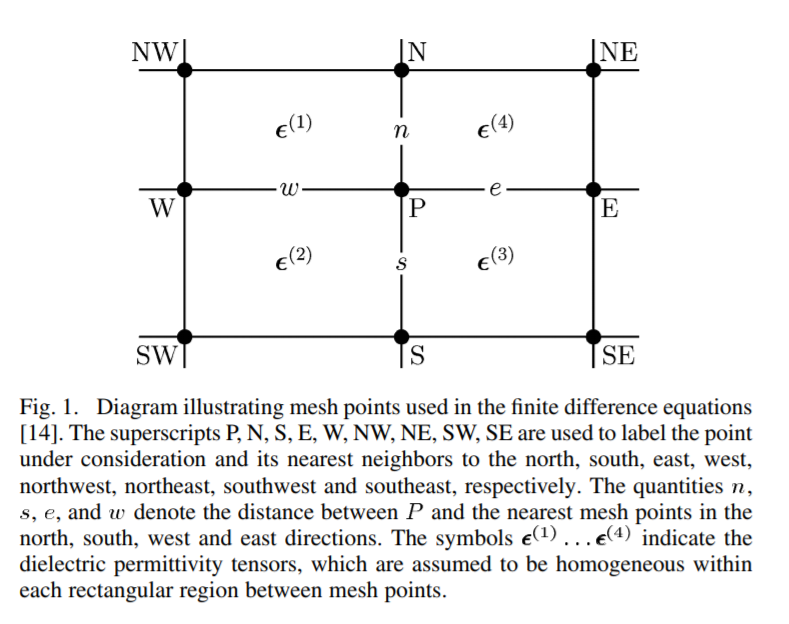
\includegraphics[scale=0.5]{grid.png}
		\caption{Fig 1}
		\label{fig:grid_points}
	\end{figure}
	
	We use the following approximations, using the convention in Fig $\ref{fig:grid_points}$.
	\begin{align*}
		\Partialsqx{H_x^p} &= \frac{H_x^w + H_x^e - 2H_x^p}{(\Delta x)^2} \\
		\Partialsqy{H_x^p} &= \frac{H_x^s + H_x^n - 2H_x^p}{(\Delta y)^2} \\
		\frac{\partial^2 H_x^p}{\partial x \partial y} &= \frac{H_x^{ne} + H_x^{sw} - H_x^{nw} - 
															H_x^{se}}{4(\Delta x)(\Delta y)}\\
		\frac{\partial^2 H_x^p}{\partial x \partial y} &= \frac{\partial^2 H_x^p}{\partial y \partial x}
	\end{align*}
	
	to discretize eqn \ref{eqn:4a*} and \ref{eqn:4b*}
	 
	\begin{align}
	\begin{split}
		\beta^2 H^x_p = \omega^2 \mu \epsilon_0 H^x_p &+ \frac{H_x^w + H_x^e - 2H_x^p}{(\Delta x)^2} + (1 - \frac{e_{yy}}{e_{zz}}) \frac{H_y^{ne} + H_y^{sw} - H_y^{nw} - H_y^{se}}{4(\Delta x)(\Delta y)} + \frac{e_{yy}}{e_{zz}} \frac{H_x^s + H_x^n - 2H_x^p}{(\Delta y)^2} 
		\label{eqn:4a_descrete}		
		\end{split}
	\end{align}
	
	\begin{align}
	\begin{split}
		\beta^2 H^y_p = \omega^2 \mu \epsilon_0 H^y_p &+ \frac{H_y^s + H_y^n - 2H_y^p}{(\Delta y)^2}  + (1 - \frac{e_{xx}}{e_{zz}}) \frac{H_x^{ne} + H_x^{sw} - H_x^{nw} - H_x^{se}}{4(\Delta x)(\Delta y)} + \frac{e_{xx}}{e_{zz}} \frac{H_y^w + H_y^e - 2H_y^p}{(\Delta x)^2} 
		\label{eqn:4b_descrete}
	\end{split}
	\end{align}
	
	The coefficients in \ref{eqn:4a_descrete} and \ref{eqn:4b_descrete} are all to be evaluated at corresponding points they are multiplied with. We have an efficient scheme for this described in the next section.\\
	
	\begin{align}
	\begin{split}
		\beta^2 H^x_p = L_1 H^x_p &+ L_2(H^x_w + H^x_e - 2H^x_p) + L_3 (H^y_{ne} + H^y_{sw} - H^y_{nw} - H^y_{se}) + L_3 (H^x_s + H^x_n - 2H^x_p) 
		\label{eqn:4a_descrete*}		
		\end{split}
	\end{align}
	
	\begin{align}
	\begin{split}
		\beta^2 H^y_p = K_1 H^y_p &+ K_2(H^y_s + H^y_n - 2H^y_p)  + K_3(H^x_{ne} + H^x_{sw} - H^x_{nw} - H^x_{se})+ K_4(H^y_w + H^y_e - 2H^y_p) 
		\label{eqn:4b_descrete*}
	\end{split}
	\end{align}
	
	\section*{Constructing the EigenMatrix - General Idea}
		
		\indent The general idea is to "unwrap" the columns of the calculation window into one long column vector and create a matrix of relationships between the elements. In the scalar wave code, we were able to execute a "brute force" method by supplying the entries of that matrix. But with the vector wave, the matrix gets large fast and we run out of memory fast. So the trick is to create a "sparse" matrix using sparse() which creates a list of entries and their values. Entries corresponding to values of 0 are effectively null and don't take up memory. \\
		\indent We will "unwrap" the computational window into a single column. So solving the transverse magnetic field becomes an eigenvalue problem. The "EigenMatrix" contains the coefficients relating the components of the transverse field. A transverse component, say $H^x$, has a value at every point of the $M \times N$ computational window. \\
		
			\begin{center}
			$H^x$ = 
			$\begin{bmatrix}
				1 & M+1 &  \hdots &  \\
				2 & M+2 &    &    \\
				3 & M+3 &  \ddots &   \vdots \\
				\vdots & \vdots &    & \vdots \\
				M &  & \hdots   & MN 
			\end{bmatrix}  
			\rightarrow
			\begin{bmatrix}
			1 \\ 2 \\ 3 \\ \vdots \\ \vdots \\ \vdots \\ nx*ny 
			\end{bmatrix}  $\\
			
		\end{center}
		
		We want to unwrap $H^x$ and $H^y$ and glue them together to get the following
		\begin{center}$
			\begin{bmatrix}
				EigenMatrix
			\end{bmatrix}
			\begin{bmatrix}
				H_x \\ H_y
			\end{bmatrix}
			\rightarrow
			\begin{bmatrix}
				EigenMatrix
			\end{bmatrix}
			\begin{bmatrix}
				H_1 \\ H_2 \\ \vdots \\ H_{MN} \\ H_{MN+1} \\ \vdots \\ H_{2MN}
			\end{bmatrix}
		$\end{center}
		 		 
		 Table \ref{table:calculation_matrix_diagram} shows a diagram for the matrices we have to construct. The inner parts, marked x, are of size $M \times N$. They are $MN$ entries describing our waveguide, consistent with the refractive index matrix. But for calculation purposes, we have to construct an $M+2 \times N+2$ size matrix because sparse() requires arguments of consistent dimensions and because we need to approximate the edge points. The padding entries are constructed using the edge entries. 
		 
		 \begin{table}[h]
		\centering
		\begin{tabular}{|c|c|c|c|c|c|c|c|c|c|}
		\hline
			 &   &   &   &   &   &   &   &   &  \\ \hline
			 & x & x & x & x & x & x & x & x &  \\ \hline
			 & x & x & x & x & x & x & x & x &  \\ \hline
			 & x & x & x & x & x & x & x & x &  \\ \hline
			 & x & x & x & x & x & x & x & x &  \\ \hline
			 & x & x & x & x & x & x & x & x &  \\ \hline
			 & x & x & x & x & x & x & x & x &  \\ \hline
			 & x & x & x & x & x & x & x & x &  \\ \hline
			 & x & x & x & x & x & x & x & x &  \\ \hline
			 &   &   &   &   &   &   &   &   &  \\ \hline
			\end{tabular}
		\caption{Calculation Matrix Diagram}
		\label{table:calculation_matrix_diagram}
	\end{table}	
	
	
		 
		\section*{Coordinate Entries}
			We see from the diagram above Table \ref{table:calculation_matrix_diagram} that the $M \times N$ entries for both the $H_x$ and $H_y$ matrices correspond to some column of the eigenMatrix. We need to keep track of the relationship between the entries in those and their corresponding entries in our unwrapped column. So lets create two $M \times N$ matrix of "coordinates" that label each entry with their corresponding entry in the column vector.\\
			
			\begin{center}
			$Hx\_coord = 
			\begin{bmatrix}
				1 & M+1 &  \hdots &  \\
				2 & M+2 &    &  \\
				3 & M+3 &  \ddots & \vdots \\
				\vdots &    &  & \vdots \\
				M &  & \hdots   & MN 
			\end{bmatrix} 
			\linebreak \linebreak
			Hy\_coord = 
			\begin{bmatrix}
				MN+1  &  \hdots &  \\
				MN+2  &    &  \\
				MN+3   \ddots & \vdots \\
				\vdots &      & \vdots \\
				... &  \hdots   & 2MN 
			\end{bmatrix} $
			\end{center}

%		\subsection*{Example}
%			Refer to Fig \ref{fig:grid_points} and Eqn \ref{eqn:H_x*}. Suppose some point $p$ under consideration corresponds %to column 12. Then the point $p$ itself for $H_x$, denote $H_x^p$, will correspond to the matrix coordinate (13,13). The $nw$ %point relative to $p$ for $H_x$, denote $H_x^{nw}$, will correspond to the matrix coordinate (13-(M+2)-1,13). The point $p$ %for $H_y$ relative to $p$, denote $H_y^p$, will correspond to the matrix coordinate (13+(M+2)(N+2), 13+(M+2)(N+2)). 

			
%		\section*{Tensor Entries}
%			Matrices containing information on our waveguide include matrices corresponding to $\epsilon_{xx}, \epsilon_{yy}, %\epsilon_{zz}, n$. Each of these are MxN matrices containing their corresponding values at each point in the waveguide. They %will be padded the same way as above turning each into a M+2 x N+2 matrix. 
			
%		\section*{The Indexer Matrix}
%			So far, our matrices have been padded along each edge and contain values we need for processing or calculating. We %now construct an indexing matrix to use for pulling these values. It will be an M+2 x N+2 matrix 
%			\begin{center}
%			$ index = 
%			\begin{bmatrix}
%				1 & M+3 &  \hdots &  \\
%				2 & M+4 &    &    \\
%				3 & M+5 &  \ddots &   \vdots \\
%				\vdots & \vdots &    & \vdots \\
%				M+2 &  & \hdots   & (M+2)(N+2) 
%			\end{bmatrix}  
%			$\\
%			\end{center}
			
%			\subsection*{Example}
%			$index(2:M-1, 2)$ contains entries corresponding to the left edge of our waveguide.
	
	
		
	
\end{document}
              